% Created by tikzDevice version 0.11 on 2018-07-02 22:35:00
% !TEX encoding = UTF-8 Unicode
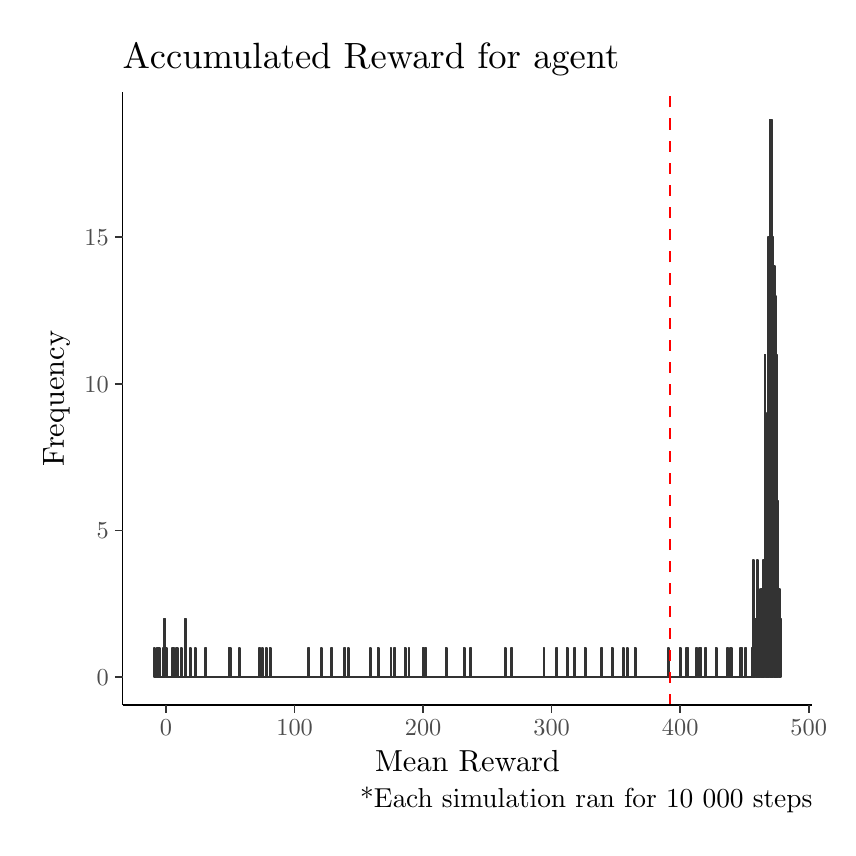
\begin{tikzpicture}[x=1pt,y=1pt]
\definecolor{fillColor}{RGB}{255,255,255}
\path[use as bounding box,fill=fillColor,fill opacity=0.00] (0,0) rectangle (289.08,289.08);
\begin{scope}
\path[clip] (  0.00,  0.00) rectangle (289.08,289.08);
\definecolor{drawColor}{RGB}{255,255,255}
\definecolor{fillColor}{RGB}{255,255,255}

\path[draw=drawColor,line width= 0.6pt,line join=round,line cap=round,fill=fillColor] (  0.00,  0.00) rectangle (289.08,289.08);
\end{scope}
\begin{scope}
\path[clip] ( 34.27, 44.27) rectangle (283.58,265.94);
\definecolor{fillColor}{RGB}{255,255,255}

\path[fill=fillColor] ( 34.27, 44.27) rectangle (283.58,265.94);
\definecolor{drawColor}{gray}{0.20}
\definecolor{fillColor}{RGB}{51,51,51}

\path[draw=drawColor,line width= 0.6pt,line join=round,fill=fillColor,fill opacity=0.80] ( 45.60, 54.35) rectangle ( 46.06, 64.95);

\path[draw=drawColor,line width= 0.6pt,line join=round,fill=fillColor,fill opacity=0.80] ( 46.06, 54.35) rectangle ( 46.53, 54.35);

\path[draw=drawColor,line width= 0.6pt,line join=round,fill=fillColor,fill opacity=0.80] ( 46.53, 54.35) rectangle ( 46.99, 64.95);

\path[draw=drawColor,line width= 0.6pt,line join=round,fill=fillColor,fill opacity=0.80] ( 46.99, 54.35) rectangle ( 47.46, 64.95);

\path[draw=drawColor,line width= 0.6pt,line join=round,fill=fillColor,fill opacity=0.80] ( 47.46, 54.35) rectangle ( 47.92, 64.95);

\path[draw=drawColor,line width= 0.6pt,line join=round,fill=fillColor,fill opacity=0.80] ( 47.92, 54.35) rectangle ( 48.39, 54.35);

\path[draw=drawColor,line width= 0.6pt,line join=round,fill=fillColor,fill opacity=0.80] ( 48.39, 54.35) rectangle ( 48.85, 54.35);

\path[draw=drawColor,line width= 0.6pt,line join=round,fill=fillColor,fill opacity=0.80] ( 48.85, 54.35) rectangle ( 49.32, 64.95);

\path[draw=drawColor,line width= 0.6pt,line join=round,fill=fillColor,fill opacity=0.80] ( 49.32, 54.35) rectangle ( 49.78, 75.56);

\path[draw=drawColor,line width= 0.6pt,line join=round,fill=fillColor,fill opacity=0.80] ( 49.78, 54.35) rectangle ( 50.24, 64.95);

\path[draw=drawColor,line width= 0.6pt,line join=round,fill=fillColor,fill opacity=0.80] ( 50.24, 54.35) rectangle ( 50.71, 54.35);

\path[draw=drawColor,line width= 0.6pt,line join=round,fill=fillColor,fill opacity=0.80] ( 50.71, 54.35) rectangle ( 51.17, 54.35);

\path[draw=drawColor,line width= 0.6pt,line join=round,fill=fillColor,fill opacity=0.80] ( 51.17, 54.35) rectangle ( 51.64, 54.35);

\path[draw=drawColor,line width= 0.6pt,line join=round,fill=fillColor,fill opacity=0.80] ( 51.64, 54.35) rectangle ( 52.10, 54.35);

\path[draw=drawColor,line width= 0.6pt,line join=round,fill=fillColor,fill opacity=0.80] ( 52.10, 54.35) rectangle ( 52.57, 64.95);

\path[draw=drawColor,line width= 0.6pt,line join=round,fill=fillColor,fill opacity=0.80] ( 52.57, 54.35) rectangle ( 53.03, 64.95);

\path[draw=drawColor,line width= 0.6pt,line join=round,fill=fillColor,fill opacity=0.80] ( 53.03, 54.35) rectangle ( 53.50, 54.35);

\path[draw=drawColor,line width= 0.6pt,line join=round,fill=fillColor,fill opacity=0.80] ( 53.50, 54.35) rectangle ( 53.96, 64.95);

\path[draw=drawColor,line width= 0.6pt,line join=round,fill=fillColor,fill opacity=0.80] ( 53.96, 54.35) rectangle ( 54.42, 64.95);

\path[draw=drawColor,line width= 0.6pt,line join=round,fill=fillColor,fill opacity=0.80] ( 54.42, 54.35) rectangle ( 54.89, 54.35);

\path[draw=drawColor,line width= 0.6pt,line join=round,fill=fillColor,fill opacity=0.80] ( 54.89, 54.35) rectangle ( 55.35, 54.35);

\path[draw=drawColor,line width= 0.6pt,line join=round,fill=fillColor,fill opacity=0.80] ( 55.35, 54.35) rectangle ( 55.82, 64.95);

\path[draw=drawColor,line width= 0.6pt,line join=round,fill=fillColor,fill opacity=0.80] ( 55.82, 54.35) rectangle ( 56.28, 54.35);

\path[draw=drawColor,line width= 0.6pt,line join=round,fill=fillColor,fill opacity=0.80] ( 56.28, 54.35) rectangle ( 56.75, 54.35);

\path[draw=drawColor,line width= 0.6pt,line join=round,fill=fillColor,fill opacity=0.80] ( 56.75, 54.35) rectangle ( 57.21, 75.56);

\path[draw=drawColor,line width= 0.6pt,line join=round,fill=fillColor,fill opacity=0.80] ( 57.21, 54.35) rectangle ( 57.68, 54.35);

\path[draw=drawColor,line width= 0.6pt,line join=round,fill=fillColor,fill opacity=0.80] ( 57.68, 54.35) rectangle ( 58.14, 54.35);

\path[draw=drawColor,line width= 0.6pt,line join=round,fill=fillColor,fill opacity=0.80] ( 58.14, 54.35) rectangle ( 58.60, 54.35);

\path[draw=drawColor,line width= 0.6pt,line join=round,fill=fillColor,fill opacity=0.80] ( 58.60, 54.35) rectangle ( 59.07, 64.95);

\path[draw=drawColor,line width= 0.6pt,line join=round,fill=fillColor,fill opacity=0.80] ( 59.07, 54.35) rectangle ( 59.53, 54.35);

\path[draw=drawColor,line width= 0.6pt,line join=round,fill=fillColor,fill opacity=0.80] ( 59.53, 54.35) rectangle ( 60.00, 54.35);

\path[draw=drawColor,line width= 0.6pt,line join=round,fill=fillColor,fill opacity=0.80] ( 60.00, 54.35) rectangle ( 60.46, 54.35);

\path[draw=drawColor,line width= 0.6pt,line join=round,fill=fillColor,fill opacity=0.80] ( 60.46, 54.35) rectangle ( 60.93, 64.95);

\path[draw=drawColor,line width= 0.6pt,line join=round,fill=fillColor,fill opacity=0.80] ( 60.93, 54.35) rectangle ( 61.39, 54.35);

\path[draw=drawColor,line width= 0.6pt,line join=round,fill=fillColor,fill opacity=0.80] ( 61.39, 54.35) rectangle ( 61.86, 54.35);

\path[draw=drawColor,line width= 0.6pt,line join=round,fill=fillColor,fill opacity=0.80] ( 61.86, 54.35) rectangle ( 62.32, 54.35);

\path[draw=drawColor,line width= 0.6pt,line join=round,fill=fillColor,fill opacity=0.80] ( 62.32, 54.35) rectangle ( 62.78, 54.35);

\path[draw=drawColor,line width= 0.6pt,line join=round,fill=fillColor,fill opacity=0.80] ( 62.78, 54.35) rectangle ( 63.25, 54.35);

\path[draw=drawColor,line width= 0.6pt,line join=round,fill=fillColor,fill opacity=0.80] ( 63.25, 54.35) rectangle ( 63.71, 54.35);

\path[draw=drawColor,line width= 0.6pt,line join=round,fill=fillColor,fill opacity=0.80] ( 63.71, 54.35) rectangle ( 64.18, 54.35);

\path[draw=drawColor,line width= 0.6pt,line join=round,fill=fillColor,fill opacity=0.80] ( 64.18, 54.35) rectangle ( 64.64, 64.95);

\path[draw=drawColor,line width= 0.6pt,line join=round,fill=fillColor,fill opacity=0.80] ( 64.64, 54.35) rectangle ( 65.11, 54.35);

\path[draw=drawColor,line width= 0.6pt,line join=round,fill=fillColor,fill opacity=0.80] ( 65.11, 54.35) rectangle ( 65.57, 54.35);

\path[draw=drawColor,line width= 0.6pt,line join=round,fill=fillColor,fill opacity=0.80] ( 65.57, 54.35) rectangle ( 66.04, 54.35);

\path[draw=drawColor,line width= 0.6pt,line join=round,fill=fillColor,fill opacity=0.80] ( 66.04, 54.35) rectangle ( 66.50, 54.35);

\path[draw=drawColor,line width= 0.6pt,line join=round,fill=fillColor,fill opacity=0.80] ( 66.50, 54.35) rectangle ( 66.96, 54.35);

\path[draw=drawColor,line width= 0.6pt,line join=round,fill=fillColor,fill opacity=0.80] ( 66.96, 54.35) rectangle ( 67.43, 54.35);

\path[draw=drawColor,line width= 0.6pt,line join=round,fill=fillColor,fill opacity=0.80] ( 67.43, 54.35) rectangle ( 67.89, 54.35);

\path[draw=drawColor,line width= 0.6pt,line join=round,fill=fillColor,fill opacity=0.80] ( 67.89, 54.35) rectangle ( 68.36, 54.35);

\path[draw=drawColor,line width= 0.6pt,line join=round,fill=fillColor,fill opacity=0.80] ( 68.36, 54.35) rectangle ( 68.82, 54.35);

\path[draw=drawColor,line width= 0.6pt,line join=round,fill=fillColor,fill opacity=0.80] ( 68.82, 54.35) rectangle ( 69.29, 54.35);

\path[draw=drawColor,line width= 0.6pt,line join=round,fill=fillColor,fill opacity=0.80] ( 69.29, 54.35) rectangle ( 69.75, 54.35);

\path[draw=drawColor,line width= 0.6pt,line join=round,fill=fillColor,fill opacity=0.80] ( 69.75, 54.35) rectangle ( 70.22, 54.35);

\path[draw=drawColor,line width= 0.6pt,line join=round,fill=fillColor,fill opacity=0.80] ( 70.22, 54.35) rectangle ( 70.68, 54.35);

\path[draw=drawColor,line width= 0.6pt,line join=round,fill=fillColor,fill opacity=0.80] ( 70.68, 54.35) rectangle ( 71.14, 54.35);

\path[draw=drawColor,line width= 0.6pt,line join=round,fill=fillColor,fill opacity=0.80] ( 71.14, 54.35) rectangle ( 71.61, 54.35);

\path[draw=drawColor,line width= 0.6pt,line join=round,fill=fillColor,fill opacity=0.80] ( 71.61, 54.35) rectangle ( 72.07, 54.35);

\path[draw=drawColor,line width= 0.6pt,line join=round,fill=fillColor,fill opacity=0.80] ( 72.07, 54.35) rectangle ( 72.54, 54.35);

\path[draw=drawColor,line width= 0.6pt,line join=round,fill=fillColor,fill opacity=0.80] ( 72.54, 54.35) rectangle ( 73.00, 64.95);

\path[draw=drawColor,line width= 0.6pt,line join=round,fill=fillColor,fill opacity=0.80] ( 73.00, 54.35) rectangle ( 73.47, 64.95);

\path[draw=drawColor,line width= 0.6pt,line join=round,fill=fillColor,fill opacity=0.80] ( 73.47, 54.35) rectangle ( 73.93, 54.35);

\path[draw=drawColor,line width= 0.6pt,line join=round,fill=fillColor,fill opacity=0.80] ( 73.93, 54.35) rectangle ( 74.40, 54.35);

\path[draw=drawColor,line width= 0.6pt,line join=round,fill=fillColor,fill opacity=0.80] ( 74.40, 54.35) rectangle ( 74.86, 54.35);

\path[draw=drawColor,line width= 0.6pt,line join=round,fill=fillColor,fill opacity=0.80] ( 74.86, 54.35) rectangle ( 75.32, 54.35);

\path[draw=drawColor,line width= 0.6pt,line join=round,fill=fillColor,fill opacity=0.80] ( 75.32, 54.35) rectangle ( 75.79, 54.35);

\path[draw=drawColor,line width= 0.6pt,line join=round,fill=fillColor,fill opacity=0.80] ( 75.79, 54.35) rectangle ( 76.25, 54.35);

\path[draw=drawColor,line width= 0.6pt,line join=round,fill=fillColor,fill opacity=0.80] ( 76.25, 54.35) rectangle ( 76.72, 64.95);

\path[draw=drawColor,line width= 0.6pt,line join=round,fill=fillColor,fill opacity=0.80] ( 76.72, 54.35) rectangle ( 77.18, 54.35);

\path[draw=drawColor,line width= 0.6pt,line join=round,fill=fillColor,fill opacity=0.80] ( 77.18, 54.35) rectangle ( 77.65, 54.35);

\path[draw=drawColor,line width= 0.6pt,line join=round,fill=fillColor,fill opacity=0.80] ( 77.65, 54.35) rectangle ( 78.11, 54.35);

\path[draw=drawColor,line width= 0.6pt,line join=round,fill=fillColor,fill opacity=0.80] ( 78.11, 54.35) rectangle ( 78.58, 54.35);

\path[draw=drawColor,line width= 0.6pt,line join=round,fill=fillColor,fill opacity=0.80] ( 78.58, 54.35) rectangle ( 79.04, 54.35);

\path[draw=drawColor,line width= 0.6pt,line join=round,fill=fillColor,fill opacity=0.80] ( 79.04, 54.35) rectangle ( 79.50, 54.35);

\path[draw=drawColor,line width= 0.6pt,line join=round,fill=fillColor,fill opacity=0.80] ( 79.50, 54.35) rectangle ( 79.97, 54.35);

\path[draw=drawColor,line width= 0.6pt,line join=round,fill=fillColor,fill opacity=0.80] ( 79.97, 54.35) rectangle ( 80.43, 54.35);

\path[draw=drawColor,line width= 0.6pt,line join=round,fill=fillColor,fill opacity=0.80] ( 80.43, 54.35) rectangle ( 80.90, 54.35);

\path[draw=drawColor,line width= 0.6pt,line join=round,fill=fillColor,fill opacity=0.80] ( 80.90, 54.35) rectangle ( 81.36, 54.35);

\path[draw=drawColor,line width= 0.6pt,line join=round,fill=fillColor,fill opacity=0.80] ( 81.36, 54.35) rectangle ( 81.83, 54.35);

\path[draw=drawColor,line width= 0.6pt,line join=round,fill=fillColor,fill opacity=0.80] ( 81.83, 54.35) rectangle ( 82.29, 54.35);

\path[draw=drawColor,line width= 0.6pt,line join=round,fill=fillColor,fill opacity=0.80] ( 82.29, 54.35) rectangle ( 82.76, 54.35);

\path[draw=drawColor,line width= 0.6pt,line join=round,fill=fillColor,fill opacity=0.80] ( 82.76, 54.35) rectangle ( 83.22, 54.35);

\path[draw=drawColor,line width= 0.6pt,line join=round,fill=fillColor,fill opacity=0.80] ( 83.22, 54.35) rectangle ( 83.68, 54.35);

\path[draw=drawColor,line width= 0.6pt,line join=round,fill=fillColor,fill opacity=0.80] ( 83.68, 54.35) rectangle ( 84.15, 64.95);

\path[draw=drawColor,line width= 0.6pt,line join=round,fill=fillColor,fill opacity=0.80] ( 84.15, 54.35) rectangle ( 84.61, 54.35);

\path[draw=drawColor,line width= 0.6pt,line join=round,fill=fillColor,fill opacity=0.80] ( 84.61, 54.35) rectangle ( 85.08, 64.95);

\path[draw=drawColor,line width= 0.6pt,line join=round,fill=fillColor,fill opacity=0.80] ( 85.08, 54.35) rectangle ( 85.54, 54.35);

\path[draw=drawColor,line width= 0.6pt,line join=round,fill=fillColor,fill opacity=0.80] ( 85.54, 54.35) rectangle ( 86.01, 54.35);

\path[draw=drawColor,line width= 0.6pt,line join=round,fill=fillColor,fill opacity=0.80] ( 86.01, 54.35) rectangle ( 86.47, 64.95);

\path[draw=drawColor,line width= 0.6pt,line join=round,fill=fillColor,fill opacity=0.80] ( 86.47, 54.35) rectangle ( 86.94, 54.35);

\path[draw=drawColor,line width= 0.6pt,line join=round,fill=fillColor,fill opacity=0.80] ( 86.94, 54.35) rectangle ( 87.40, 54.35);

\path[draw=drawColor,line width= 0.6pt,line join=round,fill=fillColor,fill opacity=0.80] ( 87.40, 54.35) rectangle ( 87.86, 64.95);

\path[draw=drawColor,line width= 0.6pt,line join=round,fill=fillColor,fill opacity=0.80] ( 87.86, 54.35) rectangle ( 88.33, 54.35);

\path[draw=drawColor,line width= 0.6pt,line join=round,fill=fillColor,fill opacity=0.80] ( 88.33, 54.35) rectangle ( 88.79, 54.35);

\path[draw=drawColor,line width= 0.6pt,line join=round,fill=fillColor,fill opacity=0.80] ( 88.79, 54.35) rectangle ( 89.26, 54.35);

\path[draw=drawColor,line width= 0.6pt,line join=round,fill=fillColor,fill opacity=0.80] ( 89.26, 54.35) rectangle ( 89.72, 54.35);

\path[draw=drawColor,line width= 0.6pt,line join=round,fill=fillColor,fill opacity=0.80] ( 89.72, 54.35) rectangle ( 90.19, 54.35);

\path[draw=drawColor,line width= 0.6pt,line join=round,fill=fillColor,fill opacity=0.80] ( 90.19, 54.35) rectangle ( 90.65, 54.35);

\path[draw=drawColor,line width= 0.6pt,line join=round,fill=fillColor,fill opacity=0.80] ( 90.65, 54.35) rectangle ( 91.12, 54.35);

\path[draw=drawColor,line width= 0.6pt,line join=round,fill=fillColor,fill opacity=0.80] ( 91.12, 54.35) rectangle ( 91.58, 54.35);

\path[draw=drawColor,line width= 0.6pt,line join=round,fill=fillColor,fill opacity=0.80] ( 91.58, 54.35) rectangle ( 92.04, 54.35);

\path[draw=drawColor,line width= 0.6pt,line join=round,fill=fillColor,fill opacity=0.80] ( 92.04, 54.35) rectangle ( 92.51, 54.35);

\path[draw=drawColor,line width= 0.6pt,line join=round,fill=fillColor,fill opacity=0.80] ( 92.51, 54.35) rectangle ( 92.97, 54.35);

\path[draw=drawColor,line width= 0.6pt,line join=round,fill=fillColor,fill opacity=0.80] ( 92.97, 54.35) rectangle ( 93.44, 54.35);

\path[draw=drawColor,line width= 0.6pt,line join=round,fill=fillColor,fill opacity=0.80] ( 93.44, 54.35) rectangle ( 93.90, 54.35);

\path[draw=drawColor,line width= 0.6pt,line join=round,fill=fillColor,fill opacity=0.80] ( 93.90, 54.35) rectangle ( 94.37, 54.35);

\path[draw=drawColor,line width= 0.6pt,line join=round,fill=fillColor,fill opacity=0.80] ( 94.37, 54.35) rectangle ( 94.83, 54.35);

\path[draw=drawColor,line width= 0.6pt,line join=round,fill=fillColor,fill opacity=0.80] ( 94.83, 54.35) rectangle ( 95.30, 54.35);

\path[draw=drawColor,line width= 0.6pt,line join=round,fill=fillColor,fill opacity=0.80] ( 95.30, 54.35) rectangle ( 95.76, 54.35);

\path[draw=drawColor,line width= 0.6pt,line join=round,fill=fillColor,fill opacity=0.80] ( 95.76, 54.35) rectangle ( 96.22, 54.35);

\path[draw=drawColor,line width= 0.6pt,line join=round,fill=fillColor,fill opacity=0.80] ( 96.22, 54.35) rectangle ( 96.69, 54.35);

\path[draw=drawColor,line width= 0.6pt,line join=round,fill=fillColor,fill opacity=0.80] ( 96.69, 54.35) rectangle ( 97.15, 54.35);

\path[draw=drawColor,line width= 0.6pt,line join=round,fill=fillColor,fill opacity=0.80] ( 97.15, 54.35) rectangle ( 97.62, 54.35);

\path[draw=drawColor,line width= 0.6pt,line join=round,fill=fillColor,fill opacity=0.80] ( 97.62, 54.35) rectangle ( 98.08, 54.35);

\path[draw=drawColor,line width= 0.6pt,line join=round,fill=fillColor,fill opacity=0.80] ( 98.08, 54.35) rectangle ( 98.55, 54.35);

\path[draw=drawColor,line width= 0.6pt,line join=round,fill=fillColor,fill opacity=0.80] ( 98.55, 54.35) rectangle ( 99.01, 54.35);

\path[draw=drawColor,line width= 0.6pt,line join=round,fill=fillColor,fill opacity=0.80] ( 99.01, 54.35) rectangle ( 99.48, 54.35);

\path[draw=drawColor,line width= 0.6pt,line join=round,fill=fillColor,fill opacity=0.80] ( 99.48, 54.35) rectangle ( 99.94, 54.35);

\path[draw=drawColor,line width= 0.6pt,line join=round,fill=fillColor,fill opacity=0.80] ( 99.94, 54.35) rectangle (100.40, 54.35);

\path[draw=drawColor,line width= 0.6pt,line join=round,fill=fillColor,fill opacity=0.80] (100.40, 54.35) rectangle (100.87, 54.35);

\path[draw=drawColor,line width= 0.6pt,line join=round,fill=fillColor,fill opacity=0.80] (100.87, 54.35) rectangle (101.33, 54.35);

\path[draw=drawColor,line width= 0.6pt,line join=round,fill=fillColor,fill opacity=0.80] (101.33, 54.35) rectangle (101.80, 64.95);

\path[draw=drawColor,line width= 0.6pt,line join=round,fill=fillColor,fill opacity=0.80] (101.80, 54.35) rectangle (102.26, 54.35);

\path[draw=drawColor,line width= 0.6pt,line join=round,fill=fillColor,fill opacity=0.80] (102.26, 54.35) rectangle (102.73, 54.35);

\path[draw=drawColor,line width= 0.6pt,line join=round,fill=fillColor,fill opacity=0.80] (102.73, 54.35) rectangle (103.19, 54.35);

\path[draw=drawColor,line width= 0.6pt,line join=round,fill=fillColor,fill opacity=0.80] (103.19, 54.35) rectangle (103.66, 54.35);

\path[draw=drawColor,line width= 0.6pt,line join=round,fill=fillColor,fill opacity=0.80] (103.66, 54.35) rectangle (104.12, 54.35);

\path[draw=drawColor,line width= 0.6pt,line join=round,fill=fillColor,fill opacity=0.80] (104.12, 54.35) rectangle (104.58, 54.35);

\path[draw=drawColor,line width= 0.6pt,line join=round,fill=fillColor,fill opacity=0.80] (104.58, 54.35) rectangle (105.05, 54.35);

\path[draw=drawColor,line width= 0.6pt,line join=round,fill=fillColor,fill opacity=0.80] (105.05, 54.35) rectangle (105.51, 54.35);

\path[draw=drawColor,line width= 0.6pt,line join=round,fill=fillColor,fill opacity=0.80] (105.51, 54.35) rectangle (105.98, 54.35);

\path[draw=drawColor,line width= 0.6pt,line join=round,fill=fillColor,fill opacity=0.80] (105.98, 54.35) rectangle (106.44, 64.95);

\path[draw=drawColor,line width= 0.6pt,line join=round,fill=fillColor,fill opacity=0.80] (106.44, 54.35) rectangle (106.91, 54.35);

\path[draw=drawColor,line width= 0.6pt,line join=round,fill=fillColor,fill opacity=0.80] (106.91, 54.35) rectangle (107.37, 54.35);

\path[draw=drawColor,line width= 0.6pt,line join=round,fill=fillColor,fill opacity=0.80] (107.37, 54.35) rectangle (107.84, 54.35);

\path[draw=drawColor,line width= 0.6pt,line join=round,fill=fillColor,fill opacity=0.80] (107.84, 54.35) rectangle (108.30, 54.35);

\path[draw=drawColor,line width= 0.6pt,line join=round,fill=fillColor,fill opacity=0.80] (108.30, 54.35) rectangle (108.76, 54.35);

\path[draw=drawColor,line width= 0.6pt,line join=round,fill=fillColor,fill opacity=0.80] (108.76, 54.35) rectangle (109.23, 54.35);

\path[draw=drawColor,line width= 0.6pt,line join=round,fill=fillColor,fill opacity=0.80] (109.23, 54.35) rectangle (109.69, 54.35);

\path[draw=drawColor,line width= 0.6pt,line join=round,fill=fillColor,fill opacity=0.80] (109.69, 54.35) rectangle (110.16, 64.95);

\path[draw=drawColor,line width= 0.6pt,line join=round,fill=fillColor,fill opacity=0.80] (110.16, 54.35) rectangle (110.62, 54.35);

\path[draw=drawColor,line width= 0.6pt,line join=round,fill=fillColor,fill opacity=0.80] (110.62, 54.35) rectangle (111.09, 54.35);

\path[draw=drawColor,line width= 0.6pt,line join=round,fill=fillColor,fill opacity=0.80] (111.09, 54.35) rectangle (111.55, 54.35);

\path[draw=drawColor,line width= 0.6pt,line join=round,fill=fillColor,fill opacity=0.80] (111.55, 54.35) rectangle (112.02, 54.35);

\path[draw=drawColor,line width= 0.6pt,line join=round,fill=fillColor,fill opacity=0.80] (112.02, 54.35) rectangle (112.48, 54.35);

\path[draw=drawColor,line width= 0.6pt,line join=round,fill=fillColor,fill opacity=0.80] (112.48, 54.35) rectangle (112.94, 54.35);

\path[draw=drawColor,line width= 0.6pt,line join=round,fill=fillColor,fill opacity=0.80] (112.94, 54.35) rectangle (113.41, 54.35);

\path[draw=drawColor,line width= 0.6pt,line join=round,fill=fillColor,fill opacity=0.80] (113.41, 54.35) rectangle (113.87, 54.35);

\path[draw=drawColor,line width= 0.6pt,line join=round,fill=fillColor,fill opacity=0.80] (113.87, 54.35) rectangle (114.34, 54.35);

\path[draw=drawColor,line width= 0.6pt,line join=round,fill=fillColor,fill opacity=0.80] (114.34, 54.35) rectangle (114.80, 64.95);

\path[draw=drawColor,line width= 0.6pt,line join=round,fill=fillColor,fill opacity=0.80] (114.80, 54.35) rectangle (115.27, 54.35);

\path[draw=drawColor,line width= 0.6pt,line join=round,fill=fillColor,fill opacity=0.80] (115.27, 54.35) rectangle (115.73, 54.35);

\path[draw=drawColor,line width= 0.6pt,line join=round,fill=fillColor,fill opacity=0.80] (115.73, 54.35) rectangle (116.20, 64.95);

\path[draw=drawColor,line width= 0.6pt,line join=round,fill=fillColor,fill opacity=0.80] (116.20, 54.35) rectangle (116.66, 54.35);

\path[draw=drawColor,line width= 0.6pt,line join=round,fill=fillColor,fill opacity=0.80] (116.66, 54.35) rectangle (117.12, 54.35);

\path[draw=drawColor,line width= 0.6pt,line join=round,fill=fillColor,fill opacity=0.80] (117.12, 54.35) rectangle (117.59, 54.35);

\path[draw=drawColor,line width= 0.6pt,line join=round,fill=fillColor,fill opacity=0.80] (117.59, 54.35) rectangle (118.05, 54.35);

\path[draw=drawColor,line width= 0.6pt,line join=round,fill=fillColor,fill opacity=0.80] (118.05, 54.35) rectangle (118.52, 54.35);

\path[draw=drawColor,line width= 0.6pt,line join=round,fill=fillColor,fill opacity=0.80] (118.52, 54.35) rectangle (118.98, 54.35);

\path[draw=drawColor,line width= 0.6pt,line join=round,fill=fillColor,fill opacity=0.80] (118.98, 54.35) rectangle (119.45, 54.35);

\path[draw=drawColor,line width= 0.6pt,line join=round,fill=fillColor,fill opacity=0.80] (119.45, 54.35) rectangle (119.91, 54.35);

\path[draw=drawColor,line width= 0.6pt,line join=round,fill=fillColor,fill opacity=0.80] (119.91, 54.35) rectangle (120.38, 54.35);

\path[draw=drawColor,line width= 0.6pt,line join=round,fill=fillColor,fill opacity=0.80] (120.38, 54.35) rectangle (120.84, 54.35);

\path[draw=drawColor,line width= 0.6pt,line join=round,fill=fillColor,fill opacity=0.80] (120.84, 54.35) rectangle (121.30, 54.35);

\path[draw=drawColor,line width= 0.6pt,line join=round,fill=fillColor,fill opacity=0.80] (121.30, 54.35) rectangle (121.77, 54.35);

\path[draw=drawColor,line width= 0.6pt,line join=round,fill=fillColor,fill opacity=0.80] (121.77, 54.35) rectangle (122.23, 54.35);

\path[draw=drawColor,line width= 0.6pt,line join=round,fill=fillColor,fill opacity=0.80] (122.23, 54.35) rectangle (122.70, 54.35);

\path[draw=drawColor,line width= 0.6pt,line join=round,fill=fillColor,fill opacity=0.80] (122.70, 54.35) rectangle (123.16, 54.35);

\path[draw=drawColor,line width= 0.6pt,line join=round,fill=fillColor,fill opacity=0.80] (123.16, 54.35) rectangle (123.63, 54.35);

\path[draw=drawColor,line width= 0.6pt,line join=round,fill=fillColor,fill opacity=0.80] (123.63, 54.35) rectangle (124.09, 64.95);

\path[draw=drawColor,line width= 0.6pt,line join=round,fill=fillColor,fill opacity=0.80] (124.09, 54.35) rectangle (124.56, 54.35);

\path[draw=drawColor,line width= 0.6pt,line join=round,fill=fillColor,fill opacity=0.80] (124.56, 54.35) rectangle (125.02, 54.35);

\path[draw=drawColor,line width= 0.6pt,line join=round,fill=fillColor,fill opacity=0.80] (125.02, 54.35) rectangle (125.48, 54.35);

\path[draw=drawColor,line width= 0.6pt,line join=round,fill=fillColor,fill opacity=0.80] (125.48, 54.35) rectangle (125.95, 54.35);

\path[draw=drawColor,line width= 0.6pt,line join=round,fill=fillColor,fill opacity=0.80] (125.95, 54.35) rectangle (126.41, 54.35);

\path[draw=drawColor,line width= 0.6pt,line join=round,fill=fillColor,fill opacity=0.80] (126.41, 54.35) rectangle (126.88, 64.95);

\path[draw=drawColor,line width= 0.6pt,line join=round,fill=fillColor,fill opacity=0.80] (126.88, 54.35) rectangle (127.34, 54.35);

\path[draw=drawColor,line width= 0.6pt,line join=round,fill=fillColor,fill opacity=0.80] (127.34, 54.35) rectangle (127.81, 54.35);

\path[draw=drawColor,line width= 0.6pt,line join=round,fill=fillColor,fill opacity=0.80] (127.81, 54.35) rectangle (128.27, 54.35);

\path[draw=drawColor,line width= 0.6pt,line join=round,fill=fillColor,fill opacity=0.80] (128.27, 54.35) rectangle (128.74, 54.35);

\path[draw=drawColor,line width= 0.6pt,line join=round,fill=fillColor,fill opacity=0.80] (128.74, 54.35) rectangle (129.20, 54.35);

\path[draw=drawColor,line width= 0.6pt,line join=round,fill=fillColor,fill opacity=0.80] (129.20, 54.35) rectangle (129.66, 54.35);

\path[draw=drawColor,line width= 0.6pt,line join=round,fill=fillColor,fill opacity=0.80] (129.66, 54.35) rectangle (130.13, 54.35);

\path[draw=drawColor,line width= 0.6pt,line join=round,fill=fillColor,fill opacity=0.80] (130.13, 54.35) rectangle (130.59, 54.35);

\path[draw=drawColor,line width= 0.6pt,line join=round,fill=fillColor,fill opacity=0.80] (130.59, 54.35) rectangle (131.06, 54.35);

\path[draw=drawColor,line width= 0.6pt,line join=round,fill=fillColor,fill opacity=0.80] (131.06, 54.35) rectangle (131.52, 64.95);

\path[draw=drawColor,line width= 0.6pt,line join=round,fill=fillColor,fill opacity=0.80] (131.52, 54.35) rectangle (131.99, 54.35);

\path[draw=drawColor,line width= 0.6pt,line join=round,fill=fillColor,fill opacity=0.80] (131.99, 54.35) rectangle (132.45, 54.35);

\path[draw=drawColor,line width= 0.6pt,line join=round,fill=fillColor,fill opacity=0.80] (132.45, 54.35) rectangle (132.92, 64.95);

\path[draw=drawColor,line width= 0.6pt,line join=round,fill=fillColor,fill opacity=0.80] (132.92, 54.35) rectangle (133.38, 54.35);

\path[draw=drawColor,line width= 0.6pt,line join=round,fill=fillColor,fill opacity=0.80] (133.38, 54.35) rectangle (133.84, 54.35);

\path[draw=drawColor,line width= 0.6pt,line join=round,fill=fillColor,fill opacity=0.80] (133.84, 54.35) rectangle (134.31, 54.35);

\path[draw=drawColor,line width= 0.6pt,line join=round,fill=fillColor,fill opacity=0.80] (134.31, 54.35) rectangle (134.77, 54.35);

\path[draw=drawColor,line width= 0.6pt,line join=round,fill=fillColor,fill opacity=0.80] (134.77, 54.35) rectangle (135.24, 54.35);

\path[draw=drawColor,line width= 0.6pt,line join=round,fill=fillColor,fill opacity=0.80] (135.24, 54.35) rectangle (135.70, 54.35);

\path[draw=drawColor,line width= 0.6pt,line join=round,fill=fillColor,fill opacity=0.80] (135.70, 54.35) rectangle (136.17, 54.35);

\path[draw=drawColor,line width= 0.6pt,line join=round,fill=fillColor,fill opacity=0.80] (136.17, 54.35) rectangle (136.63, 64.95);

\path[draw=drawColor,line width= 0.6pt,line join=round,fill=fillColor,fill opacity=0.80] (136.63, 54.35) rectangle (137.10, 54.35);

\path[draw=drawColor,line width= 0.6pt,line join=round,fill=fillColor,fill opacity=0.80] (137.10, 54.35) rectangle (137.56, 54.35);

\path[draw=drawColor,line width= 0.6pt,line join=round,fill=fillColor,fill opacity=0.80] (137.56, 54.35) rectangle (138.02, 64.95);

\path[draw=drawColor,line width= 0.6pt,line join=round,fill=fillColor,fill opacity=0.80] (138.02, 54.35) rectangle (138.49, 54.35);

\path[draw=drawColor,line width= 0.6pt,line join=round,fill=fillColor,fill opacity=0.80] (138.49, 54.35) rectangle (138.95, 54.35);

\path[draw=drawColor,line width= 0.6pt,line join=round,fill=fillColor,fill opacity=0.80] (138.95, 54.35) rectangle (139.42, 54.35);

\path[draw=drawColor,line width= 0.6pt,line join=round,fill=fillColor,fill opacity=0.80] (139.42, 54.35) rectangle (139.88, 54.35);

\path[draw=drawColor,line width= 0.6pt,line join=round,fill=fillColor,fill opacity=0.80] (139.88, 54.35) rectangle (140.35, 54.35);

\path[draw=drawColor,line width= 0.6pt,line join=round,fill=fillColor,fill opacity=0.80] (140.35, 54.35) rectangle (140.81, 54.35);

\path[draw=drawColor,line width= 0.6pt,line join=round,fill=fillColor,fill opacity=0.80] (140.81, 54.35) rectangle (141.28, 54.35);

\path[draw=drawColor,line width= 0.6pt,line join=round,fill=fillColor,fill opacity=0.80] (141.28, 54.35) rectangle (141.74, 54.35);

\path[draw=drawColor,line width= 0.6pt,line join=round,fill=fillColor,fill opacity=0.80] (141.74, 54.35) rectangle (142.20, 54.35);

\path[draw=drawColor,line width= 0.6pt,line join=round,fill=fillColor,fill opacity=0.80] (142.20, 54.35) rectangle (142.67, 54.35);

\path[draw=drawColor,line width= 0.6pt,line join=round,fill=fillColor,fill opacity=0.80] (142.67, 54.35) rectangle (143.13, 64.95);

\path[draw=drawColor,line width= 0.6pt,line join=round,fill=fillColor,fill opacity=0.80] (143.13, 54.35) rectangle (143.60, 54.35);

\path[draw=drawColor,line width= 0.6pt,line join=round,fill=fillColor,fill opacity=0.80] (143.60, 54.35) rectangle (144.06, 64.95);

\path[draw=drawColor,line width= 0.6pt,line join=round,fill=fillColor,fill opacity=0.80] (144.06, 54.35) rectangle (144.53, 54.35);

\path[draw=drawColor,line width= 0.6pt,line join=round,fill=fillColor,fill opacity=0.80] (144.53, 54.35) rectangle (144.99, 54.35);

\path[draw=drawColor,line width= 0.6pt,line join=round,fill=fillColor,fill opacity=0.80] (144.99, 54.35) rectangle (145.46, 54.35);

\path[draw=drawColor,line width= 0.6pt,line join=round,fill=fillColor,fill opacity=0.80] (145.46, 54.35) rectangle (145.92, 54.35);

\path[draw=drawColor,line width= 0.6pt,line join=round,fill=fillColor,fill opacity=0.80] (145.92, 54.35) rectangle (146.38, 54.35);

\path[draw=drawColor,line width= 0.6pt,line join=round,fill=fillColor,fill opacity=0.80] (146.38, 54.35) rectangle (146.85, 54.35);

\path[draw=drawColor,line width= 0.6pt,line join=round,fill=fillColor,fill opacity=0.80] (146.85, 54.35) rectangle (147.31, 54.35);

\path[draw=drawColor,line width= 0.6pt,line join=round,fill=fillColor,fill opacity=0.80] (147.31, 54.35) rectangle (147.78, 54.35);

\path[draw=drawColor,line width= 0.6pt,line join=round,fill=fillColor,fill opacity=0.80] (147.78, 54.35) rectangle (148.24, 54.35);

\path[draw=drawColor,line width= 0.6pt,line join=round,fill=fillColor,fill opacity=0.80] (148.24, 54.35) rectangle (148.71, 54.35);

\path[draw=drawColor,line width= 0.6pt,line join=round,fill=fillColor,fill opacity=0.80] (148.71, 54.35) rectangle (149.17, 54.35);

\path[draw=drawColor,line width= 0.6pt,line join=round,fill=fillColor,fill opacity=0.80] (149.17, 54.35) rectangle (149.64, 54.35);

\path[draw=drawColor,line width= 0.6pt,line join=round,fill=fillColor,fill opacity=0.80] (149.64, 54.35) rectangle (150.10, 54.35);

\path[draw=drawColor,line width= 0.6pt,line join=round,fill=fillColor,fill opacity=0.80] (150.10, 54.35) rectangle (150.56, 54.35);

\path[draw=drawColor,line width= 0.6pt,line join=round,fill=fillColor,fill opacity=0.80] (150.56, 54.35) rectangle (151.03, 54.35);

\path[draw=drawColor,line width= 0.6pt,line join=round,fill=fillColor,fill opacity=0.80] (151.03, 54.35) rectangle (151.49, 64.95);

\path[draw=drawColor,line width= 0.6pt,line join=round,fill=fillColor,fill opacity=0.80] (151.49, 54.35) rectangle (151.96, 54.35);

\path[draw=drawColor,line width= 0.6pt,line join=round,fill=fillColor,fill opacity=0.80] (151.96, 54.35) rectangle (152.42, 54.35);

\path[draw=drawColor,line width= 0.6pt,line join=round,fill=fillColor,fill opacity=0.80] (152.42, 54.35) rectangle (152.89, 54.35);

\path[draw=drawColor,line width= 0.6pt,line join=round,fill=fillColor,fill opacity=0.80] (152.89, 54.35) rectangle (153.35, 54.35);

\path[draw=drawColor,line width= 0.6pt,line join=round,fill=fillColor,fill opacity=0.80] (153.35, 54.35) rectangle (153.82, 54.35);

\path[draw=drawColor,line width= 0.6pt,line join=round,fill=fillColor,fill opacity=0.80] (153.82, 54.35) rectangle (154.28, 54.35);

\path[draw=drawColor,line width= 0.6pt,line join=round,fill=fillColor,fill opacity=0.80] (154.28, 54.35) rectangle (154.74, 54.35);

\path[draw=drawColor,line width= 0.6pt,line join=round,fill=fillColor,fill opacity=0.80] (154.74, 54.35) rectangle (155.21, 54.35);

\path[draw=drawColor,line width= 0.6pt,line join=round,fill=fillColor,fill opacity=0.80] (155.21, 54.35) rectangle (155.67, 54.35);

\path[draw=drawColor,line width= 0.6pt,line join=round,fill=fillColor,fill opacity=0.80] (155.67, 54.35) rectangle (156.14, 54.35);

\path[draw=drawColor,line width= 0.6pt,line join=round,fill=fillColor,fill opacity=0.80] (156.14, 54.35) rectangle (156.60, 54.35);

\path[draw=drawColor,line width= 0.6pt,line join=round,fill=fillColor,fill opacity=0.80] (156.60, 54.35) rectangle (157.07, 54.35);

\path[draw=drawColor,line width= 0.6pt,line join=round,fill=fillColor,fill opacity=0.80] (157.07, 54.35) rectangle (157.53, 54.35);

\path[draw=drawColor,line width= 0.6pt,line join=round,fill=fillColor,fill opacity=0.80] (157.53, 54.35) rectangle (158.00, 64.95);

\path[draw=drawColor,line width= 0.6pt,line join=round,fill=fillColor,fill opacity=0.80] (158.00, 54.35) rectangle (158.46, 54.35);

\path[draw=drawColor,line width= 0.6pt,line join=round,fill=fillColor,fill opacity=0.80] (158.46, 54.35) rectangle (158.92, 54.35);

\path[draw=drawColor,line width= 0.6pt,line join=round,fill=fillColor,fill opacity=0.80] (158.92, 54.35) rectangle (159.39, 54.35);

\path[draw=drawColor,line width= 0.6pt,line join=round,fill=fillColor,fill opacity=0.80] (159.39, 54.35) rectangle (159.85, 54.35);

\path[draw=drawColor,line width= 0.6pt,line join=round,fill=fillColor,fill opacity=0.80] (159.85, 54.35) rectangle (160.32, 64.95);

\path[draw=drawColor,line width= 0.6pt,line join=round,fill=fillColor,fill opacity=0.80] (160.32, 54.35) rectangle (160.78, 54.35);

\path[draw=drawColor,line width= 0.6pt,line join=round,fill=fillColor,fill opacity=0.80] (160.78, 54.35) rectangle (161.25, 54.35);

\path[draw=drawColor,line width= 0.6pt,line join=round,fill=fillColor,fill opacity=0.80] (161.25, 54.35) rectangle (161.71, 54.35);

\path[draw=drawColor,line width= 0.6pt,line join=round,fill=fillColor,fill opacity=0.80] (161.71, 54.35) rectangle (162.18, 54.35);

\path[draw=drawColor,line width= 0.6pt,line join=round,fill=fillColor,fill opacity=0.80] (162.18, 54.35) rectangle (162.64, 54.35);

\path[draw=drawColor,line width= 0.6pt,line join=round,fill=fillColor,fill opacity=0.80] (162.64, 54.35) rectangle (163.10, 54.35);

\path[draw=drawColor,line width= 0.6pt,line join=round,fill=fillColor,fill opacity=0.80] (163.10, 54.35) rectangle (163.57, 54.35);

\path[draw=drawColor,line width= 0.6pt,line join=round,fill=fillColor,fill opacity=0.80] (163.57, 54.35) rectangle (164.03, 54.35);

\path[draw=drawColor,line width= 0.6pt,line join=round,fill=fillColor,fill opacity=0.80] (164.03, 54.35) rectangle (164.50, 54.35);

\path[draw=drawColor,line width= 0.6pt,line join=round,fill=fillColor,fill opacity=0.80] (164.50, 54.35) rectangle (164.96, 54.35);

\path[draw=drawColor,line width= 0.6pt,line join=round,fill=fillColor,fill opacity=0.80] (164.96, 54.35) rectangle (165.43, 54.35);

\path[draw=drawColor,line width= 0.6pt,line join=round,fill=fillColor,fill opacity=0.80] (165.43, 54.35) rectangle (165.89, 54.35);

\path[draw=drawColor,line width= 0.6pt,line join=round,fill=fillColor,fill opacity=0.80] (165.89, 54.35) rectangle (166.35, 54.35);

\path[draw=drawColor,line width= 0.6pt,line join=round,fill=fillColor,fill opacity=0.80] (166.35, 54.35) rectangle (166.82, 54.35);

\path[draw=drawColor,line width= 0.6pt,line join=round,fill=fillColor,fill opacity=0.80] (166.82, 54.35) rectangle (167.28, 54.35);

\path[draw=drawColor,line width= 0.6pt,line join=round,fill=fillColor,fill opacity=0.80] (167.28, 54.35) rectangle (167.75, 54.35);

\path[draw=drawColor,line width= 0.6pt,line join=round,fill=fillColor,fill opacity=0.80] (167.75, 54.35) rectangle (168.21, 54.35);

\path[draw=drawColor,line width= 0.6pt,line join=round,fill=fillColor,fill opacity=0.80] (168.21, 54.35) rectangle (168.68, 54.35);

\path[draw=drawColor,line width= 0.6pt,line join=round,fill=fillColor,fill opacity=0.80] (168.68, 54.35) rectangle (169.14, 54.35);

\path[draw=drawColor,line width= 0.6pt,line join=round,fill=fillColor,fill opacity=0.80] (169.14, 54.35) rectangle (169.61, 54.35);

\path[draw=drawColor,line width= 0.6pt,line join=round,fill=fillColor,fill opacity=0.80] (169.61, 54.35) rectangle (170.07, 54.35);

\path[draw=drawColor,line width= 0.6pt,line join=round,fill=fillColor,fill opacity=0.80] (170.07, 54.35) rectangle (170.53, 54.35);

\path[draw=drawColor,line width= 0.6pt,line join=round,fill=fillColor,fill opacity=0.80] (170.53, 54.35) rectangle (171.00, 54.35);

\path[draw=drawColor,line width= 0.6pt,line join=round,fill=fillColor,fill opacity=0.80] (171.00, 54.35) rectangle (171.46, 54.35);

\path[draw=drawColor,line width= 0.6pt,line join=round,fill=fillColor,fill opacity=0.80] (171.46, 54.35) rectangle (171.93, 54.35);

\path[draw=drawColor,line width= 0.6pt,line join=round,fill=fillColor,fill opacity=0.80] (171.93, 54.35) rectangle (172.39, 54.35);

\path[draw=drawColor,line width= 0.6pt,line join=round,fill=fillColor,fill opacity=0.80] (172.39, 54.35) rectangle (172.86, 64.95);

\path[draw=drawColor,line width= 0.6pt,line join=round,fill=fillColor,fill opacity=0.80] (172.86, 54.35) rectangle (173.32, 54.35);

\path[draw=drawColor,line width= 0.6pt,line join=round,fill=fillColor,fill opacity=0.80] (173.32, 54.35) rectangle (173.79, 54.35);

\path[draw=drawColor,line width= 0.6pt,line join=round,fill=fillColor,fill opacity=0.80] (173.79, 54.35) rectangle (174.25, 54.35);

\path[draw=drawColor,line width= 0.6pt,line join=round,fill=fillColor,fill opacity=0.80] (174.25, 54.35) rectangle (174.71, 54.35);

\path[draw=drawColor,line width= 0.6pt,line join=round,fill=fillColor,fill opacity=0.80] (174.71, 54.35) rectangle (175.18, 64.95);

\path[draw=drawColor,line width= 0.6pt,line join=round,fill=fillColor,fill opacity=0.80] (175.18, 54.35) rectangle (175.64, 54.35);

\path[draw=drawColor,line width= 0.6pt,line join=round,fill=fillColor,fill opacity=0.80] (175.64, 54.35) rectangle (176.11, 54.35);

\path[draw=drawColor,line width= 0.6pt,line join=round,fill=fillColor,fill opacity=0.80] (176.11, 54.35) rectangle (176.57, 54.35);

\path[draw=drawColor,line width= 0.6pt,line join=round,fill=fillColor,fill opacity=0.80] (176.57, 54.35) rectangle (177.04, 54.35);

\path[draw=drawColor,line width= 0.6pt,line join=round,fill=fillColor,fill opacity=0.80] (177.04, 54.35) rectangle (177.50, 54.35);

\path[draw=drawColor,line width= 0.6pt,line join=round,fill=fillColor,fill opacity=0.80] (177.50, 54.35) rectangle (177.97, 54.35);

\path[draw=drawColor,line width= 0.6pt,line join=round,fill=fillColor,fill opacity=0.80] (177.97, 54.35) rectangle (178.43, 54.35);

\path[draw=drawColor,line width= 0.6pt,line join=round,fill=fillColor,fill opacity=0.80] (178.43, 54.35) rectangle (178.89, 54.35);

\path[draw=drawColor,line width= 0.6pt,line join=round,fill=fillColor,fill opacity=0.80] (178.89, 54.35) rectangle (179.36, 54.35);

\path[draw=drawColor,line width= 0.6pt,line join=round,fill=fillColor,fill opacity=0.80] (179.36, 54.35) rectangle (179.82, 54.35);

\path[draw=drawColor,line width= 0.6pt,line join=round,fill=fillColor,fill opacity=0.80] (179.82, 54.35) rectangle (180.29, 54.35);

\path[draw=drawColor,line width= 0.6pt,line join=round,fill=fillColor,fill opacity=0.80] (180.29, 54.35) rectangle (180.75, 54.35);

\path[draw=drawColor,line width= 0.6pt,line join=round,fill=fillColor,fill opacity=0.80] (180.75, 54.35) rectangle (181.22, 54.35);

\path[draw=drawColor,line width= 0.6pt,line join=round,fill=fillColor,fill opacity=0.80] (181.22, 54.35) rectangle (181.68, 54.35);

\path[draw=drawColor,line width= 0.6pt,line join=round,fill=fillColor,fill opacity=0.80] (181.68, 54.35) rectangle (182.15, 54.35);

\path[draw=drawColor,line width= 0.6pt,line join=round,fill=fillColor,fill opacity=0.80] (182.15, 54.35) rectangle (182.61, 54.35);

\path[draw=drawColor,line width= 0.6pt,line join=round,fill=fillColor,fill opacity=0.80] (182.61, 54.35) rectangle (183.07, 54.35);

\path[draw=drawColor,line width= 0.6pt,line join=round,fill=fillColor,fill opacity=0.80] (183.07, 54.35) rectangle (183.54, 54.35);

\path[draw=drawColor,line width= 0.6pt,line join=round,fill=fillColor,fill opacity=0.80] (183.54, 54.35) rectangle (184.00, 54.35);

\path[draw=drawColor,line width= 0.6pt,line join=round,fill=fillColor,fill opacity=0.80] (184.00, 54.35) rectangle (184.47, 54.35);

\path[draw=drawColor,line width= 0.6pt,line join=round,fill=fillColor,fill opacity=0.80] (184.47, 54.35) rectangle (184.93, 54.35);

\path[draw=drawColor,line width= 0.6pt,line join=round,fill=fillColor,fill opacity=0.80] (184.93, 54.35) rectangle (185.40, 54.35);

\path[draw=drawColor,line width= 0.6pt,line join=round,fill=fillColor,fill opacity=0.80] (185.40, 54.35) rectangle (185.86, 54.35);

\path[draw=drawColor,line width= 0.6pt,line join=round,fill=fillColor,fill opacity=0.80] (185.86, 54.35) rectangle (186.33, 54.35);

\path[draw=drawColor,line width= 0.6pt,line join=round,fill=fillColor,fill opacity=0.80] (186.33, 54.35) rectangle (186.79, 64.95);

\path[draw=drawColor,line width= 0.6pt,line join=round,fill=fillColor,fill opacity=0.80] (186.79, 54.35) rectangle (187.25, 54.35);

\path[draw=drawColor,line width= 0.6pt,line join=round,fill=fillColor,fill opacity=0.80] (187.25, 54.35) rectangle (187.72, 54.35);

\path[draw=drawColor,line width= 0.6pt,line join=round,fill=fillColor,fill opacity=0.80] (187.72, 54.35) rectangle (188.18, 54.35);

\path[draw=drawColor,line width= 0.6pt,line join=round,fill=fillColor,fill opacity=0.80] (188.18, 54.35) rectangle (188.65, 54.35);

\path[draw=drawColor,line width= 0.6pt,line join=round,fill=fillColor,fill opacity=0.80] (188.65, 54.35) rectangle (189.11, 54.35);

\path[draw=drawColor,line width= 0.6pt,line join=round,fill=fillColor,fill opacity=0.80] (189.11, 54.35) rectangle (189.58, 54.35);

\path[draw=drawColor,line width= 0.6pt,line join=round,fill=fillColor,fill opacity=0.80] (189.58, 54.35) rectangle (190.04, 54.35);

\path[draw=drawColor,line width= 0.6pt,line join=round,fill=fillColor,fill opacity=0.80] (190.04, 54.35) rectangle (190.51, 54.35);

\path[draw=drawColor,line width= 0.6pt,line join=round,fill=fillColor,fill opacity=0.80] (190.51, 54.35) rectangle (190.97, 54.35);

\path[draw=drawColor,line width= 0.6pt,line join=round,fill=fillColor,fill opacity=0.80] (190.97, 54.35) rectangle (191.43, 64.95);

\path[draw=drawColor,line width= 0.6pt,line join=round,fill=fillColor,fill opacity=0.80] (191.43, 54.35) rectangle (191.90, 54.35);

\path[draw=drawColor,line width= 0.6pt,line join=round,fill=fillColor,fill opacity=0.80] (191.90, 54.35) rectangle (192.36, 54.35);

\path[draw=drawColor,line width= 0.6pt,line join=round,fill=fillColor,fill opacity=0.80] (192.36, 54.35) rectangle (192.83, 54.35);

\path[draw=drawColor,line width= 0.6pt,line join=round,fill=fillColor,fill opacity=0.80] (192.83, 54.35) rectangle (193.29, 54.35);

\path[draw=drawColor,line width= 0.6pt,line join=round,fill=fillColor,fill opacity=0.80] (193.29, 54.35) rectangle (193.76, 54.35);

\path[draw=drawColor,line width= 0.6pt,line join=round,fill=fillColor,fill opacity=0.80] (193.76, 54.35) rectangle (194.22, 54.35);

\path[draw=drawColor,line width= 0.6pt,line join=round,fill=fillColor,fill opacity=0.80] (194.22, 54.35) rectangle (194.69, 54.35);

\path[draw=drawColor,line width= 0.6pt,line join=round,fill=fillColor,fill opacity=0.80] (194.69, 54.35) rectangle (195.15, 64.95);

\path[draw=drawColor,line width= 0.6pt,line join=round,fill=fillColor,fill opacity=0.80] (195.15, 54.35) rectangle (195.61, 54.35);

\path[draw=drawColor,line width= 0.6pt,line join=round,fill=fillColor,fill opacity=0.80] (195.61, 54.35) rectangle (196.08, 54.35);

\path[draw=drawColor,line width= 0.6pt,line join=round,fill=fillColor,fill opacity=0.80] (196.08, 54.35) rectangle (196.54, 54.35);

\path[draw=drawColor,line width= 0.6pt,line join=round,fill=fillColor,fill opacity=0.80] (196.54, 54.35) rectangle (197.01, 54.35);

\path[draw=drawColor,line width= 0.6pt,line join=round,fill=fillColor,fill opacity=0.80] (197.01, 54.35) rectangle (197.47, 54.35);

\path[draw=drawColor,line width= 0.6pt,line join=round,fill=fillColor,fill opacity=0.80] (197.47, 54.35) rectangle (197.94, 64.95);

\path[draw=drawColor,line width= 0.6pt,line join=round,fill=fillColor,fill opacity=0.80] (197.94, 54.35) rectangle (198.40, 54.35);

\path[draw=drawColor,line width= 0.6pt,line join=round,fill=fillColor,fill opacity=0.80] (198.40, 54.35) rectangle (198.87, 54.35);

\path[draw=drawColor,line width= 0.6pt,line join=round,fill=fillColor,fill opacity=0.80] (198.87, 54.35) rectangle (199.33, 54.35);

\path[draw=drawColor,line width= 0.6pt,line join=round,fill=fillColor,fill opacity=0.80] (199.33, 54.35) rectangle (199.79, 54.35);

\path[draw=drawColor,line width= 0.6pt,line join=round,fill=fillColor,fill opacity=0.80] (199.79, 54.35) rectangle (200.26, 54.35);

\path[draw=drawColor,line width= 0.6pt,line join=round,fill=fillColor,fill opacity=0.80] (200.26, 54.35) rectangle (200.72, 54.35);

\path[draw=drawColor,line width= 0.6pt,line join=round,fill=fillColor,fill opacity=0.80] (200.72, 54.35) rectangle (201.19, 54.35);

\path[draw=drawColor,line width= 0.6pt,line join=round,fill=fillColor,fill opacity=0.80] (201.19, 54.35) rectangle (201.65, 64.95);

\path[draw=drawColor,line width= 0.6pt,line join=round,fill=fillColor,fill opacity=0.80] (201.65, 54.35) rectangle (202.12, 54.35);

\path[draw=drawColor,line width= 0.6pt,line join=round,fill=fillColor,fill opacity=0.80] (202.12, 54.35) rectangle (202.58, 54.35);

\path[draw=drawColor,line width= 0.6pt,line join=round,fill=fillColor,fill opacity=0.80] (202.58, 54.35) rectangle (203.05, 54.35);

\path[draw=drawColor,line width= 0.6pt,line join=round,fill=fillColor,fill opacity=0.80] (203.05, 54.35) rectangle (203.51, 54.35);

\path[draw=drawColor,line width= 0.6pt,line join=round,fill=fillColor,fill opacity=0.80] (203.51, 54.35) rectangle (203.97, 54.35);

\path[draw=drawColor,line width= 0.6pt,line join=round,fill=fillColor,fill opacity=0.80] (203.97, 54.35) rectangle (204.44, 54.35);

\path[draw=drawColor,line width= 0.6pt,line join=round,fill=fillColor,fill opacity=0.80] (204.44, 54.35) rectangle (204.90, 54.35);

\path[draw=drawColor,line width= 0.6pt,line join=round,fill=fillColor,fill opacity=0.80] (204.90, 54.35) rectangle (205.37, 54.35);

\path[draw=drawColor,line width= 0.6pt,line join=round,fill=fillColor,fill opacity=0.80] (205.37, 54.35) rectangle (205.83, 54.35);

\path[draw=drawColor,line width= 0.6pt,line join=round,fill=fillColor,fill opacity=0.80] (205.83, 54.35) rectangle (206.30, 54.35);

\path[draw=drawColor,line width= 0.6pt,line join=round,fill=fillColor,fill opacity=0.80] (206.30, 54.35) rectangle (206.76, 54.35);

\path[draw=drawColor,line width= 0.6pt,line join=round,fill=fillColor,fill opacity=0.80] (206.76, 54.35) rectangle (207.23, 54.35);

\path[draw=drawColor,line width= 0.6pt,line join=round,fill=fillColor,fill opacity=0.80] (207.23, 54.35) rectangle (207.69, 64.95);

\path[draw=drawColor,line width= 0.6pt,line join=round,fill=fillColor,fill opacity=0.80] (207.69, 54.35) rectangle (208.15, 54.35);

\path[draw=drawColor,line width= 0.6pt,line join=round,fill=fillColor,fill opacity=0.80] (208.15, 54.35) rectangle (208.62, 54.35);

\path[draw=drawColor,line width= 0.6pt,line join=round,fill=fillColor,fill opacity=0.80] (208.62, 54.35) rectangle (209.08, 54.35);

\path[draw=drawColor,line width= 0.6pt,line join=round,fill=fillColor,fill opacity=0.80] (209.08, 54.35) rectangle (209.55, 54.35);

\path[draw=drawColor,line width= 0.6pt,line join=round,fill=fillColor,fill opacity=0.80] (209.55, 54.35) rectangle (210.01, 54.35);

\path[draw=drawColor,line width= 0.6pt,line join=round,fill=fillColor,fill opacity=0.80] (210.01, 54.35) rectangle (210.48, 54.35);

\path[draw=drawColor,line width= 0.6pt,line join=round,fill=fillColor,fill opacity=0.80] (210.48, 54.35) rectangle (210.94, 54.35);

\path[draw=drawColor,line width= 0.6pt,line join=round,fill=fillColor,fill opacity=0.80] (210.94, 54.35) rectangle (211.41, 64.95);

\path[draw=drawColor,line width= 0.6pt,line join=round,fill=fillColor,fill opacity=0.80] (211.41, 54.35) rectangle (211.87, 54.35);

\path[draw=drawColor,line width= 0.6pt,line join=round,fill=fillColor,fill opacity=0.80] (211.87, 54.35) rectangle (212.33, 54.35);

\path[draw=drawColor,line width= 0.6pt,line join=round,fill=fillColor,fill opacity=0.80] (212.33, 54.35) rectangle (212.80, 54.35);

\path[draw=drawColor,line width= 0.6pt,line join=round,fill=fillColor,fill opacity=0.80] (212.80, 54.35) rectangle (213.26, 54.35);

\path[draw=drawColor,line width= 0.6pt,line join=round,fill=fillColor,fill opacity=0.80] (213.26, 54.35) rectangle (213.73, 54.35);

\path[draw=drawColor,line width= 0.6pt,line join=round,fill=fillColor,fill opacity=0.80] (213.73, 54.35) rectangle (214.19, 54.35);

\path[draw=drawColor,line width= 0.6pt,line join=round,fill=fillColor,fill opacity=0.80] (214.19, 54.35) rectangle (214.66, 54.35);

\path[draw=drawColor,line width= 0.6pt,line join=round,fill=fillColor,fill opacity=0.80] (214.66, 54.35) rectangle (215.12, 54.35);

\path[draw=drawColor,line width= 0.6pt,line join=round,fill=fillColor,fill opacity=0.80] (215.12, 54.35) rectangle (215.59, 64.95);

\path[draw=drawColor,line width= 0.6pt,line join=round,fill=fillColor,fill opacity=0.80] (215.59, 54.35) rectangle (216.05, 54.35);

\path[draw=drawColor,line width= 0.6pt,line join=round,fill=fillColor,fill opacity=0.80] (216.05, 54.35) rectangle (216.51, 54.35);

\path[draw=drawColor,line width= 0.6pt,line join=round,fill=fillColor,fill opacity=0.80] (216.51, 54.35) rectangle (216.98, 64.95);

\path[draw=drawColor,line width= 0.6pt,line join=round,fill=fillColor,fill opacity=0.80] (216.98, 54.35) rectangle (217.44, 54.35);

\path[draw=drawColor,line width= 0.6pt,line join=round,fill=fillColor,fill opacity=0.80] (217.44, 54.35) rectangle (217.91, 54.35);

\path[draw=drawColor,line width= 0.6pt,line join=round,fill=fillColor,fill opacity=0.80] (217.91, 54.35) rectangle (218.37, 54.35);

\path[draw=drawColor,line width= 0.6pt,line join=round,fill=fillColor,fill opacity=0.80] (218.37, 54.35) rectangle (218.84, 54.35);

\path[draw=drawColor,line width= 0.6pt,line join=round,fill=fillColor,fill opacity=0.80] (218.84, 54.35) rectangle (219.30, 54.35);

\path[draw=drawColor,line width= 0.6pt,line join=round,fill=fillColor,fill opacity=0.80] (219.30, 54.35) rectangle (219.77, 64.95);

\path[draw=drawColor,line width= 0.6pt,line join=round,fill=fillColor,fill opacity=0.80] (219.77, 54.35) rectangle (220.23, 54.35);

\path[draw=drawColor,line width= 0.6pt,line join=round,fill=fillColor,fill opacity=0.80] (220.23, 54.35) rectangle (220.69, 54.35);

\path[draw=drawColor,line width= 0.6pt,line join=round,fill=fillColor,fill opacity=0.80] (220.69, 54.35) rectangle (221.16, 54.35);

\path[draw=drawColor,line width= 0.6pt,line join=round,fill=fillColor,fill opacity=0.80] (221.16, 54.35) rectangle (221.62, 54.35);

\path[draw=drawColor,line width= 0.6pt,line join=round,fill=fillColor,fill opacity=0.80] (221.62, 54.35) rectangle (222.09, 54.35);

\path[draw=drawColor,line width= 0.6pt,line join=round,fill=fillColor,fill opacity=0.80] (222.09, 54.35) rectangle (222.55, 54.35);

\path[draw=drawColor,line width= 0.6pt,line join=round,fill=fillColor,fill opacity=0.80] (222.55, 54.35) rectangle (223.02, 54.35);

\path[draw=drawColor,line width= 0.6pt,line join=round,fill=fillColor,fill opacity=0.80] (223.02, 54.35) rectangle (223.48, 54.35);

\path[draw=drawColor,line width= 0.6pt,line join=round,fill=fillColor,fill opacity=0.80] (223.48, 54.35) rectangle (223.95, 54.35);

\path[draw=drawColor,line width= 0.6pt,line join=round,fill=fillColor,fill opacity=0.80] (223.95, 54.35) rectangle (224.41, 54.35);

\path[draw=drawColor,line width= 0.6pt,line join=round,fill=fillColor,fill opacity=0.80] (224.41, 54.35) rectangle (224.87, 54.35);

\path[draw=drawColor,line width= 0.6pt,line join=round,fill=fillColor,fill opacity=0.80] (224.87, 54.35) rectangle (225.34, 54.35);

\path[draw=drawColor,line width= 0.6pt,line join=round,fill=fillColor,fill opacity=0.80] (225.34, 54.35) rectangle (225.80, 54.35);

\path[draw=drawColor,line width= 0.6pt,line join=round,fill=fillColor,fill opacity=0.80] (225.80, 54.35) rectangle (226.27, 54.35);

\path[draw=drawColor,line width= 0.6pt,line join=round,fill=fillColor,fill opacity=0.80] (226.27, 54.35) rectangle (226.73, 54.35);

\path[draw=drawColor,line width= 0.6pt,line join=round,fill=fillColor,fill opacity=0.80] (226.73, 54.35) rectangle (227.20, 54.35);

\path[draw=drawColor,line width= 0.6pt,line join=round,fill=fillColor,fill opacity=0.80] (227.20, 54.35) rectangle (227.66, 54.35);

\path[draw=drawColor,line width= 0.6pt,line join=round,fill=fillColor,fill opacity=0.80] (227.66, 54.35) rectangle (228.13, 54.35);

\path[draw=drawColor,line width= 0.6pt,line join=round,fill=fillColor,fill opacity=0.80] (228.13, 54.35) rectangle (228.59, 54.35);

\path[draw=drawColor,line width= 0.6pt,line join=round,fill=fillColor,fill opacity=0.80] (228.59, 54.35) rectangle (229.05, 54.35);

\path[draw=drawColor,line width= 0.6pt,line join=round,fill=fillColor,fill opacity=0.80] (229.05, 54.35) rectangle (229.52, 54.35);

\path[draw=drawColor,line width= 0.6pt,line join=round,fill=fillColor,fill opacity=0.80] (229.52, 54.35) rectangle (229.98, 54.35);

\path[draw=drawColor,line width= 0.6pt,line join=round,fill=fillColor,fill opacity=0.80] (229.98, 54.35) rectangle (230.45, 54.35);

\path[draw=drawColor,line width= 0.6pt,line join=round,fill=fillColor,fill opacity=0.80] (230.45, 54.35) rectangle (230.91, 54.35);

\path[draw=drawColor,line width= 0.6pt,line join=round,fill=fillColor,fill opacity=0.80] (230.91, 54.35) rectangle (231.38, 54.35);

\path[draw=drawColor,line width= 0.6pt,line join=round,fill=fillColor,fill opacity=0.80] (231.38, 54.35) rectangle (231.84, 64.95);

\path[draw=drawColor,line width= 0.6pt,line join=round,fill=fillColor,fill opacity=0.80] (231.84, 54.35) rectangle (232.31, 54.35);

\path[draw=drawColor,line width= 0.6pt,line join=round,fill=fillColor,fill opacity=0.80] (232.31, 54.35) rectangle (232.77, 54.35);

\path[draw=drawColor,line width= 0.6pt,line join=round,fill=fillColor,fill opacity=0.80] (232.77, 54.35) rectangle (233.23, 54.35);

\path[draw=drawColor,line width= 0.6pt,line join=round,fill=fillColor,fill opacity=0.80] (233.23, 54.35) rectangle (233.70, 54.35);

\path[draw=drawColor,line width= 0.6pt,line join=round,fill=fillColor,fill opacity=0.80] (233.70, 54.35) rectangle (234.16, 54.35);

\path[draw=drawColor,line width= 0.6pt,line join=round,fill=fillColor,fill opacity=0.80] (234.16, 54.35) rectangle (234.63, 54.35);

\path[draw=drawColor,line width= 0.6pt,line join=round,fill=fillColor,fill opacity=0.80] (234.63, 54.35) rectangle (235.09, 54.35);

\path[draw=drawColor,line width= 0.6pt,line join=round,fill=fillColor,fill opacity=0.80] (235.09, 54.35) rectangle (235.56, 54.35);

\path[draw=drawColor,line width= 0.6pt,line join=round,fill=fillColor,fill opacity=0.80] (235.56, 54.35) rectangle (236.02, 64.95);

\path[draw=drawColor,line width= 0.6pt,line join=round,fill=fillColor,fill opacity=0.80] (236.02, 54.35) rectangle (236.49, 54.35);

\path[draw=drawColor,line width= 0.6pt,line join=round,fill=fillColor,fill opacity=0.80] (236.49, 54.35) rectangle (236.95, 54.35);

\path[draw=drawColor,line width= 0.6pt,line join=round,fill=fillColor,fill opacity=0.80] (236.95, 54.35) rectangle (237.41, 54.35);

\path[draw=drawColor,line width= 0.6pt,line join=round,fill=fillColor,fill opacity=0.80] (237.41, 54.35) rectangle (237.88, 54.35);

\path[draw=drawColor,line width= 0.6pt,line join=round,fill=fillColor,fill opacity=0.80] (237.88, 54.35) rectangle (238.34, 64.95);

\path[draw=drawColor,line width= 0.6pt,line join=round,fill=fillColor,fill opacity=0.80] (238.34, 54.35) rectangle (238.81, 64.95);

\path[draw=drawColor,line width= 0.6pt,line join=round,fill=fillColor,fill opacity=0.80] (238.81, 54.35) rectangle (239.27, 54.35);

\path[draw=drawColor,line width= 0.6pt,line join=round,fill=fillColor,fill opacity=0.80] (239.27, 54.35) rectangle (239.74, 54.35);

\path[draw=drawColor,line width= 0.6pt,line join=round,fill=fillColor,fill opacity=0.80] (239.74, 54.35) rectangle (240.20, 54.35);

\path[draw=drawColor,line width= 0.6pt,line join=round,fill=fillColor,fill opacity=0.80] (240.20, 54.35) rectangle (240.67, 54.35);

\path[draw=drawColor,line width= 0.6pt,line join=round,fill=fillColor,fill opacity=0.80] (240.67, 54.35) rectangle (241.13, 54.35);

\path[draw=drawColor,line width= 0.6pt,line join=round,fill=fillColor,fill opacity=0.80] (241.13, 54.35) rectangle (241.59, 54.35);

\path[draw=drawColor,line width= 0.6pt,line join=round,fill=fillColor,fill opacity=0.80] (241.59, 54.35) rectangle (242.06, 64.95);

\path[draw=drawColor,line width= 0.6pt,line join=round,fill=fillColor,fill opacity=0.80] (242.06, 54.35) rectangle (242.52, 54.35);

\path[draw=drawColor,line width= 0.6pt,line join=round,fill=fillColor,fill opacity=0.80] (242.52, 54.35) rectangle (242.99, 64.95);

\path[draw=drawColor,line width= 0.6pt,line join=round,fill=fillColor,fill opacity=0.80] (242.99, 54.35) rectangle (243.45, 64.95);

\path[draw=drawColor,line width= 0.6pt,line join=round,fill=fillColor,fill opacity=0.80] (243.45, 54.35) rectangle (243.92, 54.35);

\path[draw=drawColor,line width= 0.6pt,line join=round,fill=fillColor,fill opacity=0.80] (243.92, 54.35) rectangle (244.38, 54.35);

\path[draw=drawColor,line width= 0.6pt,line join=round,fill=fillColor,fill opacity=0.80] (244.38, 54.35) rectangle (244.85, 54.35);

\path[draw=drawColor,line width= 0.6pt,line join=round,fill=fillColor,fill opacity=0.80] (244.85, 54.35) rectangle (245.31, 64.95);

\path[draw=drawColor,line width= 0.6pt,line join=round,fill=fillColor,fill opacity=0.80] (245.31, 54.35) rectangle (245.77, 54.35);

\path[draw=drawColor,line width= 0.6pt,line join=round,fill=fillColor,fill opacity=0.80] (245.77, 54.35) rectangle (246.24, 54.35);

\path[draw=drawColor,line width= 0.6pt,line join=round,fill=fillColor,fill opacity=0.80] (246.24, 54.35) rectangle (246.70, 54.35);

\path[draw=drawColor,line width= 0.6pt,line join=round,fill=fillColor,fill opacity=0.80] (246.70, 54.35) rectangle (247.17, 54.35);

\path[draw=drawColor,line width= 0.6pt,line join=round,fill=fillColor,fill opacity=0.80] (247.17, 54.35) rectangle (247.63, 54.35);

\path[draw=drawColor,line width= 0.6pt,line join=round,fill=fillColor,fill opacity=0.80] (247.63, 54.35) rectangle (248.10, 54.35);

\path[draw=drawColor,line width= 0.6pt,line join=round,fill=fillColor,fill opacity=0.80] (248.10, 54.35) rectangle (248.56, 54.35);

\path[draw=drawColor,line width= 0.6pt,line join=round,fill=fillColor,fill opacity=0.80] (248.56, 54.35) rectangle (249.03, 64.95);

\path[draw=drawColor,line width= 0.6pt,line join=round,fill=fillColor,fill opacity=0.80] (249.03, 54.35) rectangle (249.49, 54.35);

\path[draw=drawColor,line width= 0.6pt,line join=round,fill=fillColor,fill opacity=0.80] (249.49, 54.35) rectangle (249.95, 54.35);

\path[draw=drawColor,line width= 0.6pt,line join=round,fill=fillColor,fill opacity=0.80] (249.95, 54.35) rectangle (250.42, 54.35);

\path[draw=drawColor,line width= 0.6pt,line join=round,fill=fillColor,fill opacity=0.80] (250.42, 54.35) rectangle (250.88, 54.35);

\path[draw=drawColor,line width= 0.6pt,line join=round,fill=fillColor,fill opacity=0.80] (250.88, 54.35) rectangle (251.35, 54.35);

\path[draw=drawColor,line width= 0.6pt,line join=round,fill=fillColor,fill opacity=0.80] (251.35, 54.35) rectangle (251.81, 54.35);

\path[draw=drawColor,line width= 0.6pt,line join=round,fill=fillColor,fill opacity=0.80] (251.81, 54.35) rectangle (252.28, 54.35);

\path[draw=drawColor,line width= 0.6pt,line join=round,fill=fillColor,fill opacity=0.80] (252.28, 54.35) rectangle (252.74, 54.35);

\path[draw=drawColor,line width= 0.6pt,line join=round,fill=fillColor,fill opacity=0.80] (252.74, 54.35) rectangle (253.21, 64.95);

\path[draw=drawColor,line width= 0.6pt,line join=round,fill=fillColor,fill opacity=0.80] (253.21, 54.35) rectangle (253.67, 54.35);

\path[draw=drawColor,line width= 0.6pt,line join=round,fill=fillColor,fill opacity=0.80] (253.67, 54.35) rectangle (254.13, 64.95);

\path[draw=drawColor,line width= 0.6pt,line join=round,fill=fillColor,fill opacity=0.80] (254.13, 54.35) rectangle (254.60, 64.95);

\path[draw=drawColor,line width= 0.6pt,line join=round,fill=fillColor,fill opacity=0.80] (254.60, 54.35) rectangle (255.06, 54.35);

\path[draw=drawColor,line width= 0.6pt,line join=round,fill=fillColor,fill opacity=0.80] (255.06, 54.35) rectangle (255.53, 54.35);

\path[draw=drawColor,line width= 0.6pt,line join=round,fill=fillColor,fill opacity=0.80] (255.53, 54.35) rectangle (255.99, 54.35);

\path[draw=drawColor,line width= 0.6pt,line join=round,fill=fillColor,fill opacity=0.80] (255.99, 54.35) rectangle (256.46, 54.35);

\path[draw=drawColor,line width= 0.6pt,line join=round,fill=fillColor,fill opacity=0.80] (256.46, 54.35) rectangle (256.92, 54.35);

\path[draw=drawColor,line width= 0.6pt,line join=round,fill=fillColor,fill opacity=0.80] (256.92, 54.35) rectangle (257.39, 54.35);

\path[draw=drawColor,line width= 0.6pt,line join=round,fill=fillColor,fill opacity=0.80] (257.39, 54.35) rectangle (257.85, 64.95);

\path[draw=drawColor,line width= 0.6pt,line join=round,fill=fillColor,fill opacity=0.80] (257.85, 54.35) rectangle (258.31, 64.95);

\path[draw=drawColor,line width= 0.6pt,line join=round,fill=fillColor,fill opacity=0.80] (258.31, 54.35) rectangle (258.78, 54.35);

\path[draw=drawColor,line width= 0.6pt,line join=round,fill=fillColor,fill opacity=0.80] (258.78, 54.35) rectangle (259.24, 54.35);

\path[draw=drawColor,line width= 0.6pt,line join=round,fill=fillColor,fill opacity=0.80] (259.24, 54.35) rectangle (259.71, 64.95);

\path[draw=drawColor,line width= 0.6pt,line join=round,fill=fillColor,fill opacity=0.80] (259.71, 54.35) rectangle (260.17, 54.35);

\path[draw=drawColor,line width= 0.6pt,line join=round,fill=fillColor,fill opacity=0.80] (260.17, 54.35) rectangle (260.64, 54.35);

\path[draw=drawColor,line width= 0.6pt,line join=round,fill=fillColor,fill opacity=0.80] (260.64, 54.35) rectangle (261.10, 54.35);

\path[draw=drawColor,line width= 0.6pt,line join=round,fill=fillColor,fill opacity=0.80] (261.10, 54.35) rectangle (261.57, 54.35);

\path[draw=drawColor,line width= 0.6pt,line join=round,fill=fillColor,fill opacity=0.80] (261.57, 54.35) rectangle (262.03, 64.95);

\path[draw=drawColor,line width= 0.6pt,line join=round,fill=fillColor,fill opacity=0.80] (262.03, 54.35) rectangle (262.49, 96.77);

\path[draw=drawColor,line width= 0.6pt,line join=round,fill=fillColor,fill opacity=0.80] (262.49, 54.35) rectangle (262.96, 64.95);

\path[draw=drawColor,line width= 0.6pt,line join=round,fill=fillColor,fill opacity=0.80] (262.96, 54.35) rectangle (263.42, 75.56);

\path[draw=drawColor,line width= 0.6pt,line join=round,fill=fillColor,fill opacity=0.80] (263.42, 54.35) rectangle (263.89, 96.77);

\path[draw=drawColor,line width= 0.6pt,line join=round,fill=fillColor,fill opacity=0.80] (263.89, 54.35) rectangle (264.35, 86.17);

\path[draw=drawColor,line width= 0.6pt,line join=round,fill=fillColor,fill opacity=0.80] (264.35, 54.35) rectangle (264.82, 54.35);

\path[draw=drawColor,line width= 0.6pt,line join=round,fill=fillColor,fill opacity=0.80] (264.82, 54.35) rectangle (265.28, 86.17);

\path[draw=drawColor,line width= 0.6pt,line join=round,fill=fillColor,fill opacity=0.80] (265.28, 54.35) rectangle (265.75, 75.56);

\path[draw=drawColor,line width= 0.6pt,line join=round,fill=fillColor,fill opacity=0.80] (265.75, 54.35) rectangle (266.21, 96.77);

\path[draw=drawColor,line width= 0.6pt,line join=round,fill=fillColor,fill opacity=0.80] (266.21, 54.35) rectangle (266.67,171.02);

\path[draw=drawColor,line width= 0.6pt,line join=round,fill=fillColor,fill opacity=0.80] (266.67, 54.35) rectangle (267.14,128.59);

\path[draw=drawColor,line width= 0.6pt,line join=round,fill=fillColor,fill opacity=0.80] (267.14, 54.35) rectangle (267.60,149.80);

\path[draw=drawColor,line width= 0.6pt,line join=round,fill=fillColor,fill opacity=0.80] (267.60, 54.35) rectangle (268.07,213.44);

\path[draw=drawColor,line width= 0.6pt,line join=round,fill=fillColor,fill opacity=0.80] (268.07, 54.35) rectangle (268.53,255.87);

\path[draw=drawColor,line width= 0.6pt,line join=round,fill=fillColor,fill opacity=0.80] (268.53, 54.35) rectangle (269.00,255.87);

\path[draw=drawColor,line width= 0.6pt,line join=round,fill=fillColor,fill opacity=0.80] (269.00, 54.35) rectangle (269.46,213.44);

\path[draw=drawColor,line width= 0.6pt,line join=round,fill=fillColor,fill opacity=0.80] (269.46, 54.35) rectangle (269.93,202.84);

\path[draw=drawColor,line width= 0.6pt,line join=round,fill=fillColor,fill opacity=0.80] (269.93, 54.35) rectangle (270.39,192.23);

\path[draw=drawColor,line width= 0.6pt,line join=round,fill=fillColor,fill opacity=0.80] (270.39, 54.35) rectangle (270.85,171.02);

\path[draw=drawColor,line width= 0.6pt,line join=round,fill=fillColor,fill opacity=0.80] (270.85, 54.35) rectangle (271.32,117.99);

\path[draw=drawColor,line width= 0.6pt,line join=round,fill=fillColor,fill opacity=0.80] (271.32, 54.35) rectangle (271.78, 86.17);

\path[draw=drawColor,line width= 0.6pt,line join=round,fill=fillColor,fill opacity=0.80] (271.78, 54.35) rectangle (272.25, 75.56);
\definecolor{drawColor}{RGB}{255,0,0}

\path[draw=drawColor,line width= 0.6pt,dash pattern=on 4pt off 4pt ,line join=round] (232.02, 44.27) -- (232.02,265.94);
\end{scope}
\begin{scope}
\path[clip] (  0.00,  0.00) rectangle (289.08,289.08);
\definecolor{drawColor}{RGB}{0,0,0}

\path[draw=drawColor,line width= 0.6pt,line join=round] ( 34.27, 44.27) --
	( 34.27,265.94);
\end{scope}
\begin{scope}
\path[clip] (  0.00,  0.00) rectangle (289.08,289.08);
\definecolor{drawColor}{gray}{0.30}

\node[text=drawColor,anchor=base east,inner sep=0pt, outer sep=0pt, scale=  0.88] at ( 29.32, 51.32) {0};

\node[text=drawColor,anchor=base east,inner sep=0pt, outer sep=0pt, scale=  0.88] at ( 29.32,104.35) {5};

\node[text=drawColor,anchor=base east,inner sep=0pt, outer sep=0pt, scale=  0.88] at ( 29.32,157.38) {10};

\node[text=drawColor,anchor=base east,inner sep=0pt, outer sep=0pt, scale=  0.88] at ( 29.32,210.41) {15};
\end{scope}
\begin{scope}
\path[clip] (  0.00,  0.00) rectangle (289.08,289.08);
\definecolor{drawColor}{gray}{0.20}

\path[draw=drawColor,line width= 0.6pt,line join=round] ( 31.52, 54.35) --
	( 34.27, 54.35);

\path[draw=drawColor,line width= 0.6pt,line join=round] ( 31.52,107.38) --
	( 34.27,107.38);

\path[draw=drawColor,line width= 0.6pt,line join=round] ( 31.52,160.41) --
	( 34.27,160.41);

\path[draw=drawColor,line width= 0.6pt,line join=round] ( 31.52,213.44) --
	( 34.27,213.44);
\end{scope}
\begin{scope}
\path[clip] (  0.00,  0.00) rectangle (289.08,289.08);
\definecolor{drawColor}{RGB}{0,0,0}

\path[draw=drawColor,line width= 0.6pt,line join=round] ( 34.27, 44.27) --
	(283.58, 44.27);
\end{scope}
\begin{scope}
\path[clip] (  0.00,  0.00) rectangle (289.08,289.08);
\definecolor{drawColor}{gray}{0.20}

\path[draw=drawColor,line width= 0.6pt,line join=round] ( 50.01, 41.52) --
	( 50.01, 44.27);

\path[draw=drawColor,line width= 0.6pt,line join=round] ( 96.46, 41.52) --
	( 96.46, 44.27);

\path[draw=drawColor,line width= 0.6pt,line join=round] (142.90, 41.52) --
	(142.90, 44.27);

\path[draw=drawColor,line width= 0.6pt,line join=round] (189.34, 41.52) --
	(189.34, 44.27);

\path[draw=drawColor,line width= 0.6pt,line join=round] (235.79, 41.52) --
	(235.79, 44.27);

\path[draw=drawColor,line width= 0.6pt,line join=round] (282.23, 41.52) --
	(282.23, 44.27);
\end{scope}
\begin{scope}
\path[clip] (  0.00,  0.00) rectangle (289.08,289.08);
\definecolor{drawColor}{gray}{0.30}

\node[text=drawColor,anchor=base,inner sep=0pt, outer sep=0pt, scale=  0.88] at ( 50.01, 33.26) {0};

\node[text=drawColor,anchor=base,inner sep=0pt, outer sep=0pt, scale=  0.88] at ( 96.46, 33.26) {100};

\node[text=drawColor,anchor=base,inner sep=0pt, outer sep=0pt, scale=  0.88] at (142.90, 33.26) {200};

\node[text=drawColor,anchor=base,inner sep=0pt, outer sep=0pt, scale=  0.88] at (189.34, 33.26) {300};

\node[text=drawColor,anchor=base,inner sep=0pt, outer sep=0pt, scale=  0.88] at (235.79, 33.26) {400};

\node[text=drawColor,anchor=base,inner sep=0pt, outer sep=0pt, scale=  0.88] at (282.23, 33.26) {500};
\end{scope}
\begin{scope}
\path[clip] (  0.00,  0.00) rectangle (289.08,289.08);
\definecolor{drawColor}{RGB}{0,0,0}

\node[text=drawColor,anchor=base,inner sep=0pt, outer sep=0pt, scale=  1.10] at (158.92, 20.18) {Mean Reward};
\end{scope}
\begin{scope}
\path[clip] (  0.00,  0.00) rectangle (289.08,289.08);
\definecolor{drawColor}{RGB}{0,0,0}

\node[text=drawColor,rotate= 90.00,anchor=base,inner sep=0pt, outer sep=0pt, scale=  1.10] at ( 13.08,155.11) {Frequency};
\end{scope}
\begin{scope}
\path[clip] (  0.00,  0.00) rectangle (289.08,289.08);
\definecolor{drawColor}{RGB}{0,0,0}

\node[text=drawColor,anchor=base west,inner sep=0pt, outer sep=0pt, scale=  1.32] at ( 34.27,274.49) {Accumulated Reward for agent};
\end{scope}
\begin{scope}
\path[clip] (  0.00,  0.00) rectangle (289.08,289.08);
\definecolor{drawColor}{RGB}{0,0,0}

\node[text=drawColor,anchor=base east,inner sep=0pt, outer sep=0pt, scale=  0.99] at (283.58,  7.44) {*Each simulation ran for 10 000 steps};
\end{scope}
\end{tikzpicture}
